\subsubsection{Pregled cena usluga}
\label{subsubsec:vozni park}
\begin{itemize}
  \item \textbf{Kratak opis}: Računovođa vodi računa o cenana usluga i mogućim popustima

  \item \textbf{Učesnici}:
    \begin{itemize}
    \item Računovođa.
    \item Kandidat.
    \end{itemize}
  \item \textbf{Preduslovi}:
    \begin{itemize}
    \item  Kandidat želi da se upiše u auto školu.
    \end{itemize}
  \item \textbf{Postuslovi}:
      \begin{itemize}
      \item  Kandidatu je određena cena obuke.
      \end{itemize}
  \item \textbf{Osnovni tok}:
      \begin{enumerate}
        \item Kandidat donosi osnovne podatke računovođi.
        \item Računovođa saopštava osnovnu cenu obuke.
        \item Računovođa određuje popust za datog kandidata.
        \item Računovođa saopštava cenu obuke sa popustom.
        \item Kandidat nastavlja sa upisom.
      \end{enumerate}

  \item \textbf{Alternativni tokovi}:
      \begin{itemize}
        \item A1. \textbf{Kandidat ne prihvata cenu obuke:}
        Kandidatu ne odgovara cena obuke. Proces se prekida.
      \end{itemize}

      
  \item \textbf{Dodatne informacije}:
      \begin{itemize}
        \item Računovođa oređuje popust na osnovu socijalno ekonomskog statusa i na osnovu pripadnosti društveno osetljivim grupama.
      \end{itemize}
\end{itemize}

\begin{figure}[H]
  \begin{center}
      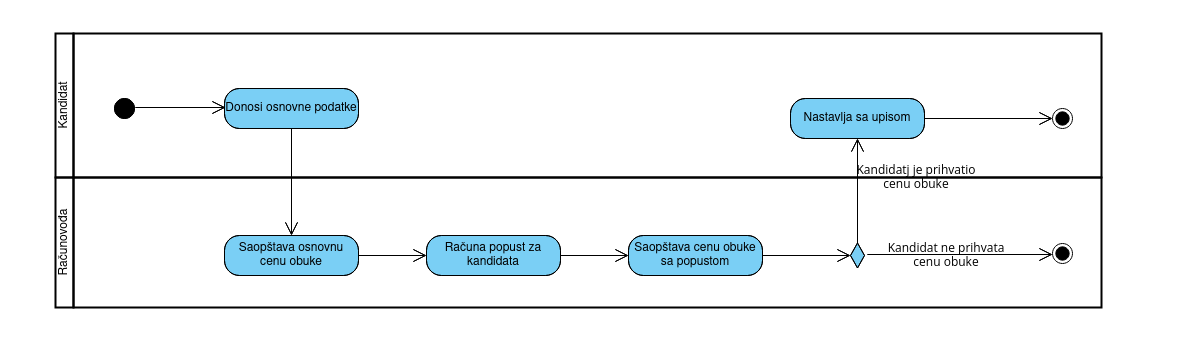
\includegraphics[width=140mm, height=70mm]{Diagrams/dijagram_aktivnosti_cena_obuke.png}
  \end{center}
  \caption {Dijagram aktivnosti - Pregled cena usluga}
  \label{activity_pregled_cena_usluga}

\end{figure}

